\documentclass[proposal]{softeng}

\usepackage{times}
\usepackage{outline}
\usepackage{ulem}
\usepackage{mdwlist}

\title{MSc Project Proposal}
\author{Mike McClurg}
\organisation{University of Oxford}
\college{Kellogg College}
\award{Software Engineering}

\date{\today}

\begin{document}

\maketitle

\begin{abstract}

  %% You should include a 100 to 200 word abstract.

  Object mocking is a technique to assist programmers in writing unit
  tests, by replacing hard-to-test dependencies with ``mock''
  implementations of those dependencies. A mock object allows the
  developer to set certain expectations about how the system under test
  will interact with the dependency, and then verify that these
  expectations hold true at the end of the test. While this technique
  was developed as a test design pattern for object oriented
  languages, it can also useful for functional programming languages,
  especially for applications in which hard-to-test side effects can't
  easily be factored out of pure functions. This dissertation will
  explore the current state of the art tools and techniques for unit
  testing and mock object generation in object oriented languages. It
  will make the case that these techniques can be of use in functional
  programming languages, and it will describe the implementation and
  use of a new mocking library for the OCaml programming language.

  % ... Alas, functional languages are not immune to ...

\end{abstract}

\section{Area of study}

%% You should provide a brief account of the application domain: the
%% situation that you are going to explore, the software that you are
%% going to develop, or the problem that you wish to address.  This
%% section should be one or two pages long.

Testing is an important part of software development. Software tests
are often categorised as either system, component, or unit
tests. These categories represent a spectrum of granularity. Systems
tests represent the broadest granularity, and are meant to test the
entire system as a whole. On the other end of the spectrum are unit
tests, which test functionality at the finest level of granularity:
typically a method or function. Component tests sit somewhere in
between the two ends of the spectrum, and might test interactions
between modules or classes of an application, or perhaps the
interaction between a web server and a database. A system test may
require a test environment that is an exact replica of the production
system, whereas a unit test may be run on the developer's workstation
each time the software is rebuilt.

%% Systems tests test the entire system as a whole; for instance, a
%% system test for a web application may duplicate an entire
%% production environment to test the interaction of system components
%% from end to end. (System tests are meant to test the entire system
%% as a whole; for instance, a system test of a server virtualization
%% system might install the virtualization system on two physical
%% hosts, install a virtual machine on one of the hosts, and then
%% assert that this virtual machine can successfully migrate to the
%% other physical host.)  Component tests are meant to test the
%% interactions between individual components of the system. These are
%% distinct from systems test, which test all the components of the
%% system

Recent trends in Agile development, such as Continuous Integration
\cite{humble:continuous} and Test Driven Development \cite{beck:tdd},
have placed a greater emphasis on unit testing. Consequentially, many
tools and libraries have been developed to assist programmers in
writing these tests. Many of these libraries, such as JUnit
\cite{www:junit} for Java, NUnit \cite{www:nunit} for .NET, and OUnit
\cite{www:ounit} for OCaml, follow the xUnit patterns of test
development described by Meszaros \cite{meszaros:xunit}. This family
of libraries typically provides a set of convenient assertion
functions to help the user write test cases, annotations to help
organise these test cases into larger test suites, and test harnesses
to handle test running and status reporting.

A common problem with writing unit tests is that, for various reasons,
some code is just hard to test. This is often the case when the
depended-on component (DOC) of the system under test (SUT) performs
some side-effecting operation that is not valid in the test scenario,
or is otherwise impossible to run from within the test
harness.

It would be helpful here to step back and examine a simple motivating
example. Consider how one would write unit tests for the user
interface of a nuclear missile launch system. This hypothetical
missile launch system has built-in safeties to prevent accidentally
firing missiles. These safeties may involve, say, two users initiating
a launch sequence by pressing two big red buttons, on opposite sides
of a room, within a specific time window. We would like to test that
the launch interface triggers the missile launch system on the correct
inputs, but not on incorrect inputs. Figure \ref{fig:missile_orig}
illustrates the two components of this system. In this example, the
system under test (SUT) is the missile launch interface, while the
depended-on component (DOC) is the missile launcher. Launching
missiles is the side-effect that we would like to avoid during our
testing; the missile launching system is an example of hard-to-test
code.

\begin{figure}
  \centering
  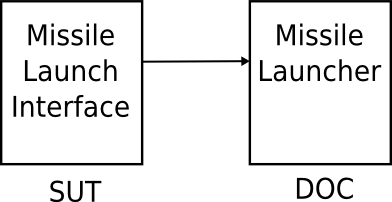
\includegraphics[scale=.45]{img/missile_launch1.png}
  \caption{A motivating example: how to test a missile launcher
    interface?}
  \label{fig:missile_orig}
\end{figure}

Hard-to-test code requires one to refactor the SUT so that the
hard-to-test DOC can be replaced by a test double
\cite{meszaros:xunit}. This test double might be a dummy object (such
as Java's \verb|null| object, which fulfils the DOC's interface but
doesn't implement it), a test spy (which implements the DOC's
interface and simply records each method access for later analysis),
or a mock object. Mocks are a powerful type of test double which allow
implementations to be easily specified in the test cases themselves;
they also allow ``expectations'' about the way the SUT interacts with
the DOC to be expressed and later verified. Mocks are a powerful tool
which allow one to write concise, maintainable unit tests that are
less prone to ``brittle test syndrome'' than tests written differently
\cite{meszaros:xunit}. JMock \cite{www:jmock} is an excellent example
of a mocking library that automatically generates mock objects and
provides a very convenient method for specifying and evaluating
expectations on those mocks. Figure \ref{fig:taxonomy} shows the
taxonomy of test doubles. We are concerned with mock objects, which
are outlined in blue.

%% \begin{figure}
%%   \centering
%%   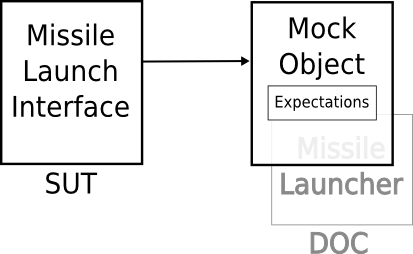
\includegraphics[scale=.45]{img/missile_launch2.png}
%%   \caption{Mocking the missile launcher}
%%   \label{fig:missile2}
%% \end{figure}

\begin{figure}
  \centering
  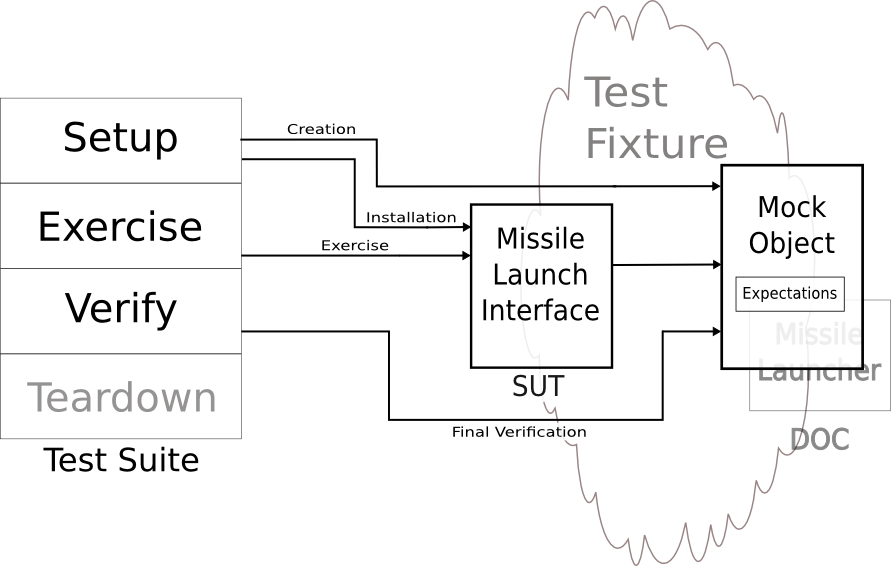
\includegraphics[scale=.45]{img/missile_launch3.png}
  \caption{Mock object in the context of a test and test fixture
    (adapted from \cite{meszaros:xunit})}
  \label{fig:missile_mock}
\end{figure}

\begin{figure}
  \centering
  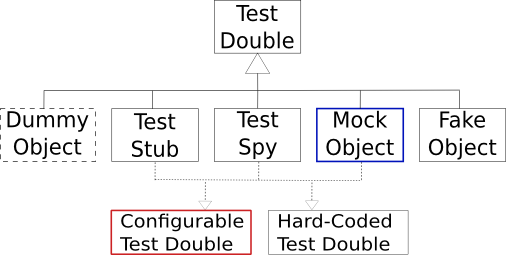
\includegraphics[scale=.7]{img/test_double_taxonomy.png}
  \caption{Test double taxonomy (adapted from \cite{meszaros:xunit})}
  \label{fig:taxonomy}
\end{figure}

Figure \ref{fig:missile_mock} shows missile launcher example again, but
this time with a mock object replacing the original DOC. We see that
the test suite on the left performs the operations setup, exercise,
verify, and teardown while performing tests against the SUT (missile
launch interface). In the setup phase, the test suite creates the mock
object to replace the hard-to-test DOC (missile launcher). In the
creation of the mock, the test suite specifies a number of
expectations on how that mock should act, and how the SUT should
interact witih it. For instance, one test in the test suite may expect
that only after the two launch buttons on the interface are pressed
within $N$ milliseconds, the mock missile launcher receives the
``fire'' signal from the interface. After creating a mock, the test
then installs it into the SUT as a replacement for the DOC. The test
suite then exercises the test, and verifies that the mock's
expectations were satisfied during the test. The teardown phase of the
test is not demonstrated in this figure.

% Psuedo language for expectations on the missile launcher:
% Mock mockLauncher = new Mock(MissileLauncher);
% final BigDecimal MILLISBETWEENPRESS = new BigDecimal(999);
% context.checking(new Expectations() {{
%    oneOf(mockLauncher).signalLaunch(); will(returnValue(timeOfFirstPress));
%    oneOf(mockLauncher).signalLaunch(); will(returnValue(timeOfSecondPress));
%    allowing(BigDecimal
% }});
% context.assertionIsSatisfied();
% mockLauncher.expects(twice()).method(``signalLaunch'');
% mockLauncher.

% Now I should transition to talking about unit testing in functional
% programming languages

While most of the literature about unit testing and tools for unit
testing are written about testing object oriented languages, many of
these techniques also apply directly to functional programming
languages. HUnit \cite{www:hunit} and OUnit \cite{www:ounit} provide
unit testing frameworks for Haskell and OCaml, respectively. Kaputt
\cite{www:kaputt} is another unit testing framework for OCaml which
provides a variety of modules to assist in writing tests, as well as
prototypical mocking combinators to assist in manually writing mock
functions. Unfortunately, Kaputt's mocking functions require the user
to manually write out mocks, and Kaputt doesn't provide the powerful
expectation specification mechanisms that other mocking libraries like
JMock \cite{www:jmock} provide.
% (Somewhere I need to talk about why Kaputt's mocking is not sufficiently powerful.)

% Talk about quickcheck, factoring pure from side-effecting code.
In fact, functional programming languages often lend themselves to
additional testing techniques that aren't as easily applied to object
oriented languages. Haskell and, to a lesser extent, OCaml, both have
access to a tool called QuickCheck \cite{canou:ocaml_random_test}
\cite{claessen:quickcheck}, which test the properties of functions by
generating random test inputs based on the type of the function under
test. Haskell unit testing in particular benefits from Haskell's
purity, or freedom from side effects. Because all side effects in
Haskell must be encapsulated in monads, it is easy to identify pure,
side effect free functions for which tests that don't require test
doubles are easy to write. Most object oriented languages don't
provide this level of surety about the lack of side effects in a
function.

%% Talk about how the above techniques don't always apply simply
%% because of the nature of the application domain or the way in which
%% a legacy application was written, and bring us back to why and how
%% mocks could be useful in a functional programming language such as
%% OCaml.

Most functional languages don't enforce the level of purity that
Haskell does. OCaml, for instance, does allow for mutable state, and
doesn't force the programmer to separate side effecting code from
referentially transparent code. So while OCaml encourages good
programming practices such as separating referentially transparent
code from side effecting code, and minimising mutable state, it
doesn't enforce these practices. Furthermore, some application domains
are by their nature more prone to requiring a large portion of the
code base to produce or deal with side effects. In situations like
these, the ability to easily swap out hard-to-test dependencies with
mechanically generated test doubles is very important to the developer
who wants to write readable test cases quickly and easily.

\section{Proposed work}

%% You should explain what you intend to do, how you propose to do it,
%% and what you expect to achieve in terms of outcomes.  It should be
%% clear from your explanation:
%% \begin{itemize}
%% \item which aspects of the situation, system, or problem that you intend
%%   to address---the intended scope of your project;
%% \item which principles, methods, tools, or techniques you intend to
%%   apply;
%% \item what you expect to be able to report, and how this will serve to
%%   demonstrate your mastery of the subject.
%% \end{itemize}
%% This section also should be one or two pages long.

The main output of my project will be MoCaml, a mocking library for
OCaml which mechanically generates mocks and provides an expectation
framework which will make it easy for developers to write test cases
using these mocks. This library should integrate well with existing
OCaml unit testing libraries, and will likely build upon them.

As mentioned previously, the Kaputt unit testing library does have a
set of helper functions for manually creating mocks, and for
performing limited expectation checking on these mocks. In the test
double taxonomy described in Figure \ref{fig:taxonomy}, the type of
mock that a developer could write using Kaputt would be a ``hard-coded
mock.'' The Kaputt library is a step in the right direction for OCaml,
but it is incomplete when compared against libraries such as Java's
JMock, which have automatic mock generation capabilities, as well as a
convenient and powerful syntax for specifying expectations. Kaputt's
existing mocking helper functions may be useful as a starting point
for automatically generating mocks in MoCaml, though the Kaputt mock
library is not required for implementing MoCaml.

The automatic mock object generation capabilities of the JMock library
are made possible by the Java language's reflection capabilities. At
run time, the JMock library can inspect the types of the objects being
mocked, and generate on-the-fly a replica of that object's
interface. This interface is then connected to JMock's expectations
framework so that it can be instrumented by the test case. The
reflection property that makes this possible in Java is unfortunately
not present in OCaml. While the OCaml language lacks reflection, it
does have a very powerful preprocessor and macro facility called
camlp4 \cite{www:reading_camlp4}. As a preprocessor, camlp4 is much
more akin to Lisp's syntax macros than to C's preprocessor directives,
providing the ability to write syntax extensions as well as direct
access to a program's untyped AST. Camlp4 is powerful enough to do
compile-time mock generation, as well as to allow us to write just
enough extra syntax to make writing and using mock and expectations
convenient.

In contrast to Kaputt, MoCaml will offer the developer the ability to
write ``configurable mocks,'' as shown in the test double taxonomy in
the red box. By allowing the programmer to write automatically
generated, configurable mock modules, the MoCaml library will provide
much greater convenience for writing test cases than the mocking
library provided by Kaputt, and will greatly reduce the time it takes
for developers to write tests using the mock module test pattern.

%% - explanation of the technical difficulties overcome in writing library
%% - comparison of mocking with Kaputt to mocking with MoCaml
%% - detailed treatment of mocking technique and how it can be usefully applied to OCaml
%% Specifically what my library will do. ``Three things'' that it does.

\section{Project plan}

%% You should explain the order in which you will address the various
%% aspects of the work, a realistic allocation of time to each task, and
%% the dates by which each task should be completed.  You should list key
%% milestones and interim outputs or results, and explain what actions
%% would be taken if some of these could not be achieved: what would you
%% do instead?   This section should be between half a page and perhaps a
%% whole page in length.

As a rough estimate, I expect that the time spent on my dissertation
will break down as follows.

\begin{itemize*}
  \item Literature survey (5\%)
  \item MoCaml library implementation (35\%)
  \item Dissertation (60\%)
\end{itemize*}

While I am very interested in producing a polished, high-quality
library for testing with mock modules in OCaml, I realise that the
primary purpose of this effort is to produce a thorough dissertation
that demonstrates my master of the subject matter. For this reason, I
have budgeted only 35\% of my total time for coding the library
itself, and the rest of the time for writing my dissertation. I hope
that my work over the next six months will proceed as follows. Please
note that I am hoping to submit my thesis in Trinity Term 2013, on 6
September.
\\

\begin{center}
\begin{tabular}{l | c | c | c | p{3cm}}
  \bf{Work item} & \bf{Est. effort} & \bf{Start date} & \bf{Finish date} & \bf{Comment} \\
  \hline
  \sout{Literature survey} & \sout{1 wk} & \sout{8 Jan 13} & \sout{15 Jan 13} &
    \sout{Complete} \\
  Intro/background chapters & 6 wks & 25 Feb 13 & 7 Apr 13 & In progress \\
  Application chapters & 12 wks & 8 Apr 13 & 23 Jun & \\
  Reflection chapter & 4 wks & 24 Jun & 28 Jul & \\
  Final revisions & 4 wks & 29 Jul & 26 Aug & \\
  \hline
  Write MoCaml library & 16 wks left & 26 Sep 12 & 17 Jun & Estimates are for working concurrently on dissertation \\
\end{tabular}
\end{center}

While the table above shows that I began work on the MoCaml library in
September 2012, the work has been sporadic since then; I expect that
from this point, the library will take another three months to
complete. The first few chapters of my dissertation will not depend on
a completed library, and so can be completed simultaneously. I have
accounted for this concurrent effort in my estimates above.

I believe that the estimates above are acheivable, and that they leave
room for slippage, because much of the dissertation will be
independent of having completed the MoCaml library. If unforseen
circumstances prevent me from spending as much time on this work as I
would like to, I will still be able to complete my work in time for
the next deadline in the Michaelmas Term.

\section{Dissertation structure}

%% You should describe the broad organisation of your dissertation, an
%% outline table of contents, including chapter headings and subheadings
%% would be fine.

My dissertation will follow this outline. I expect that the
Application chapter will likely be split into two chapters.

\begin{outline}
\item Introduction
  \begin{outline}
  \item Motivation of this dissertation
  \item Objectives and expected contribution
  \item Organisation
  \end{outline}
\item Background
  \begin{outline}
  \item Unit testing, and problem with hard-to-test dependencies
  \item The test double pattern, especially mocks
  \item Functional languages, specifically testing
  \item State of current tools for testing, especially in
    functional languages, and again, especially in OCaml
  \item Existing tools, capabilities in OCaml that I can base my library on
  \end{outline}
\item Application (this may be split into two chapters)
  \begin{outline}
  \item Brief explanation of camlp4 preprocessing technique that
    will be used (camlp4 is a bit of a black art!)
  \item Treatment of OCaml's unique module structure and type
    system, which is both very powerful for this application, and at
    the same time difficult to work around.
  \item Explanation of my mock and expectation implementation. The
    techniques that I produce for my library will be the main
    academic contribution of my dissertation.
  \item Comparison of tests written using a) no mocking technique,
    b) Kaputt mocking library, c) MoCaml mocking
    library. Demonstrate pros and cons of each technique, and
    describe when one would prefer one over the other.
    % Might want an evaluation chapter...
  \end{outline}
\item Reflection
  \begin{outline}
  \item Examples of using MoCaml library. There will probably be running
    examples throughout the dissertation.
  \item Stretch goal: case study of MoCaml used in industry. My team
    at work will hopefully find this library useful. If we can make
    use of it in time for my dissertation, it would be good to
    describe how we used it.
  \end{outline}
\end{outline}

\nocite{*}
\bibliographystyle{plain}
\bibliography{bibliography}

\end{document}
